\documentclass{beamer}
\mode<presentation>{
  \usetheme{Boadilla}
  \usefonttheme[onlylarge]{structurebold}
  \usefonttheme[stillsansseriflarge]{serif}
  \setbeamerfont*{frametitle}{size=\normalsize,series=\bfseries}
  % \setbeamertemplate{navigation symbols}{}
  \setbeamercovered{transparent}
}
\usepackage[english]{babel}
\usepackage[latin1]{inputenc}
\usepackage{times}
\usepackage[T1]{fontenc}
\usepackage{amsmath}
\usepackage{amssymb}
\usepackage{esint}
\usepackage{hyperref}
\usepackage{tikz}
\usepackage{xkeyval}
\usepackage{xargs}
\usepackage{verbatim}
\usetikzlibrary{
  arrows,
  calc,
  decorations.pathmorphing,
  decorations.pathreplacing,
  decorations.markings,
  fadings,
  positioning,
  shapes
}

\mode<handout>{
  \usepackage{pgfpages}
  \pgfpagesuselayout{4 on 1}[a4paper,landscape,border shrink=5mm]
  \setbeamercolor{background canvas}{bg=black!10}
}

\newcommand\pgfmathsinandcos[3]{%
  \pgfmathsetmacro#1{sin(#3)}%
  \pgfmathsetmacro#2{cos(#3)}%
}
\newcommand\LongitudePlane[3][current plane]{%
  \pgfmathsinandcos\sinEl\cosEl{#2} % elevation
  \pgfmathsinandcos\sint\cost{#3} % azimuth
  \tikzset{#1/.estyle={cm={\cost,\sint*\sinEl,0,\cosEl,(0,0)}}}
}
\newcommand\LatitudePlane[3][current plane]{%
  \pgfmathsinandcos\sinEl\cosEl{#2} % elevation
  \pgfmathsinandcos\sint\cost{#3} % latitude
  \pgfmathsetmacro\yshift{\cosEl*\sint}
  \tikzset{#1/.estyle={cm={\cost,0,0,\cost*\sinEl,(0,\yshift)}}} %
}
\newcommand\DrawLongitudeCircle[2][1]{
  \LongitudePlane{\angEl}{#2}
  \tikzset{current plane/.prefix style={scale=#1}}
  % angle of "visibility"
  \pgfmathsetmacro\angVis{atan(sin(#2)*cos(\angEl)/sin(\angEl))} %
  \draw[current plane] (\angVis:1) arc (\angVis:\angVis+180:1);
  \draw[current plane,dashed] (\angVis-180:1) arc (\angVis-180:\angVis:1);
}
\newcommand\DrawLatitudeCircleArrow[2][1]{
  \LatitudePlane{\angEl}{#2}
  \tikzset{current plane/.prefix style={scale=#1}}
  \pgfmathsetmacro\sinVis{sin(#2)/cos(#2)*sin(\angEl)/cos(\angEl)}
  % angle of "visibility"
  \pgfmathsetmacro\angVis{asin(min(1,max(\sinVis,-1)))}
  \draw[current plane,decoration={markings, mark=at position 0.6 with {\arrow{<}}},postaction={decorate},line width=.6mm] (\angVis:1) arc (\angVis:-\angVis-180:1);
  \draw[current plane,dashed,line width=.6mm] (180-\angVis:1) arc (180-\angVis:\angVis:1);
}
\newcommand\DrawLatitudeCircle[2][1]{
  \LatitudePlane{\angEl}{#2}
  \tikzset{current plane/.prefix style={scale=#1}}
  \pgfmathsetmacro\sinVis{sin(#2)/cos(#2)*sin(\angEl)/cos(\angEl)}
  % angle of "visibility"
  \pgfmathsetmacro\angVis{asin(min(1,max(\sinVis,-1)))}
  \draw[current plane] (\angVis:1) arc (\angVis:-\angVis-180:1);
  \draw[current plane,dashed] (180-\angVis:1) arc (180-\angVis:\angVis:1);
}
\newcommand\coil[1]{
  {\rh * cos(\t * pi r)}, {\apart * (2 * #1 + \t) + \rv * sin(\t * pi r)}
}
\makeatletter
\define@key{DrawFromCenter}{style}[{->}]{
  \tikzset{DrawFromCenterPlane/.style={#1}}
}
\define@key{DrawFromCenter}{r}[1]{
  \def\@R{#1}
}
\define@key{DrawFromCenter}{center}[(0, 0)]{
  \def\@Center{#1}
}
\define@key{DrawFromCenter}{theta}[0]{
  \def\@Theta{#1}
}
\define@key{DrawFromCenter}{phi}[0]{
  \def\@Phi{#1}
}
\presetkeys{DrawFromCenter}{style, r, center, theta, phi}{}
\newcommand*\DrawFromCenter[1][]{
  \setkeys{DrawFromCenter}{#1}{
    \pgfmathsinandcos\sint\cost{\@Theta}
    \pgfmathsinandcos\sinp\cosp{\@Phi}
    \pgfmathsinandcos\sinA\cosA{\angEl}
    \pgfmathsetmacro\DX{\@R*\cost*\cosp}
    \pgfmathsetmacro\DY{\@R*(\cost*\sinp*\sinA+\sint*\cosA)}
    \draw[DrawFromCenterPlane] \@Center -- ++(\DX, \DY);
  }
}
\newcommand*\DrawFromCenterText[2][]{
  \setkeys{DrawFromCenter}{#1}{
    \pgfmathsinandcos\sint\cost{\@Theta}
    \pgfmathsinandcos\sinp\cosp{\@Phi}
    \pgfmathsinandcos\sinA\cosA{\angEl}
    \pgfmathsetmacro\DX{\@R*\cost*\cosp}
    \pgfmathsetmacro\DY{\@R*(\cost*\sinp*\sinA+\sint*\cosA)}
    \draw[DrawFromCenterPlane] \@Center -- ++(\DX, \DY) node {#2};
  }
}
\makeatother

% not mandatory, but I though it was better to set it blank
\setbeamertemplate{headline}{}
\def\beamer@entrycode{\vspace{-\headheight}}

\tikzstyle{snakearrow} = [decorate, decoration={pre length=0.2cm,
  post length=0.2cm, snake, amplitude=.4mm,
  segment length=2mm},thick, ->]

%% document-wide tikz options and styles

\tikzset{%
  >=latex, % option for nice arrows
  inner sep=0pt,%
  outer sep=2pt,%
  mark coordinate/.style={inner sep=0pt,outer sep=0pt,minimum size=3pt,
    fill=black,circle}%
}
\def\timeleft{15:00->14:55}

\title[Doppler-free spectroscopy\hspace{2em}\tiny{\timeleft}]{Doppler-free spectroscopy using saturated absorption}
\author{Yichao Yu}
\institute{MIT}

\begin{document}

\begin{frame}{}
  \titlepage
\end{frame}

% Intro
\def\timeleft{14:55->14:20}
\begin{frame}{Introduction}
  \begin{block}{}
    \begin{itemize}[<+->]
    \item
      Saturated absorption.
    \item
      Precise spectrum measurement.
    \item
      Frequency stabilization and locking.
    \end{itemize}
  \end{block}
\end{frame}

\def\timeleft{14:20->13:50}
\begin{frame}
  \tableofcontents
\end{frame}

\def\timeleft{13:50->11:40}
% Theory
\section{Doppler broadening and saturated absorption.}
\begin{frame}{Doppler broadening and spectral hole burning.}
  \begin{columns}
    \column{6cm}
    \begin{block}{}
      \begin{itemize}[<+->]
      \item
        Natural line width.
      \item
        Doppler broadening.
        \[ \Delta f=\frac{v}{c}f_0\approx100MHz \]
      \item
        Cooling.
      \item
        He-Ne spectral whole burning discovered by Bennett in 1962.\only<+->{}
      \item
        Saturated absorption in vapor cell.
      \end{itemize}
    \end{block}
    \column{6cm}
    \visible<4-> {
      \begin{tikzpicture}[scale=.8]
        \only<4> {
          \draw[smooth,domain=-2.5:2.5] plot function{2*exp(-x**2)};
        }
        \only<5-> {
          \draw[smooth,domain=-2.5:2.5,dashed] plot function{2*exp(-x**2)};
          \draw[smooth,domain=-2.5:2.5] plot function{2*exp(-x**2)-1.2*exp(-x**2 * 40)};
        }
        \draw[->,black] (-3,0) -- (3,0) node[right] {$f$};
        \draw[->,black] (0,0) -- (0,3);
      \end{tikzpicture}
    }
  \end{columns}
\end{frame}

\begin{frame}{Saturated absorption.}
  \begin{columns}
    \column{6cm}
    \begin{block}{}
      \begin{itemize}[<+->]
      \item
        Saturation intensity.\only<+->{}
      \item
        Saturate absorption with two beams. Velocity selecting and Lamb dip.
      \item
        Crossover peaks.
      \end{itemize}
    \end{block}
    \column{6cm}
    \begin{tikzpicture}[scale=.8]
      \visible<4-> {
        \draw[line width=2] (0, 7) -- (6, 7) node[right] {$E_2$};
        \draw[red, line width=2] (0, 6) -- (6, 6) node[right, black] {$E_{laser}$};
        \draw[<->, blue, line width=2] (2, 6) -- (2, 7);
        \draw[<->, blue, line width=2] (2, 6) -- (2, 5);
        \path (2, 6.5) node[right] {$+\Delta E_{doppler}$};
        \path (2, 5.5) node[right] {$-\Delta E_{doppler}$};
      }
      \draw[line width=2] (0, 5) -- (6, 5) node[right] {\only<-3>{$E$}\only<4->{$E_1$}};
      \draw[line width=2] (0, 0) -- (6, 0) node[right] {$G$};

      \only<1> {
        \draw[line width=6, red, ->] (0, 2) -- (5, 2)
        node[right, black, align=center] {weak\\beam};
        \draw[line width=2, red, ->] (2, 2) -- (4, 1)
        node[right, black, align=center] {scatter};
        \draw[line width=1.5, fill=black] (0.5, 0) circle (0.2);
        \draw[line width=1.5, fill=black] (1.0, 0) circle (0.2);
        \draw[line width=1.5, fill=black] (1.5, 0) circle (0.2);
        \draw[line width=1.5, fill=black] (2.0, 0) circle (0.2);
        \draw[line width=1.5, fill=black] (2.5, 0) circle (0.2);
        \draw[line width=1.5, fill=black] (3.0, 0) circle (0.2);
        \draw[line width=1.5, fill=black] (3.5, 0) circle (0.2);
        \draw[line width=1.5, fill=black] (4.0, 0) circle (0.2);
        \draw[line width=1.5, fill=black] (4.5, 0) circle (0.2);
        \draw[line width=1.5, fill=black] (5.0, 0) circle (0.2);
        \draw[line width=1.5, fill=black] (5.5, 0) circle (0.2);
        \draw[line width=1.5, fill=black] (3, 5) circle (0.2);
      }

      \only<2-3> {
        \draw[line width=18, red, ->] (0, 2) -- (5, 2)
        node[right, black, align=center] {strong\\beam};
        \draw[line width=6, red, ->] (1, 2) -- (2.5, .5)
        node[right, black, align=center] {scatter};
        \draw[line width=1.5, fill=black] (0.5, 5) circle (0.2);
        \draw[line width=1.5, fill=black] (0.5, 0) circle (0.2);
        \draw[line width=1.5, fill=black] (1.5, 5) circle (0.2);
        \draw[line width=1.5, fill=black] (1.5, 0) circle (0.2);
        \draw[line width=1.5, fill=black] (2.5, 5) circle (0.2);
        \draw[line width=1.5, fill=black] (2.5, 0) circle (0.2);
        \draw[line width=1.5, fill=black] (3.5, 5) circle (0.2);
        \draw[line width=1.5, fill=black] (3.5, 0) circle (0.2);
        \draw[line width=1.5, fill=black] (4.5, 5) circle (0.2);
        \draw[line width=1.5, fill=black] (4.5, 0) circle (0.2);
        \draw[line width=1.5, fill=black] (5.5, 5) circle (0.2);
        \draw[line width=1.5, fill=black] (5.5, 0) circle (0.2);
      }
      \only<3> {
        \draw[line width=4, red, ->] (6, 4) -- (1, 4)
        node[left, black, align=center] {second\\beam};
      }
    \end{tikzpicture}
  \end{columns}
\end{frame}

\def\timeleft{10:00 -> 7:30}
% apparatus
\section{Apparatus and measurement.}
\begin{frame}{Apparatus.}
  \begin{center}
    \begin{tikzpicture}[scale=.8]
      \draw[line width=2] (1, -.2) rectangle (2, .2) node[above] {Diode laser};
      \draw (-.5, -0.5) -- ++(-1, 1) -- ++(-.2, -.2) -- ++(1, -1) -- ++(.2, .2);

      \visible<2-> {
        \draw[red, line width=2] (1, 0) -- (-1, 0) -- ++(-.3, -.1) -- (-7, -.1);
        \draw[red, line width=.7] (-7, -.1) -- (-9, -.1);
        \draw[red, line width=2] (-7, -.1) -- (-1.36, 3.24);
      }
      \visible<3-> {
        \draw[red, line width=1] (-1, 0) -- (-1, 3);
        \draw[red, line width=1] (-1.3, -.1) -- (-1.3, 3.2);
        \draw[red, line width=.7] (-1.27, 3.18) -- (-6.94, -.16) -- (-8.074, -.828);
        \draw[red, line width=.7] (-.97, 2.98) -- (-6.7, -.4) -- (-7.846, -1.076) node[below, black] {measure power};
      }

      \visible<4-> {
        \draw[line width=1, dashed] (-.3, -.3) -- (.3, .3);
        \draw[red, dashed, line width=1] (0, 0) -- (0, -1) node[black, below] {FP cavity};
      }

      \draw[line width=2] (-.7, 2.8) -- (-1.6, 3.4);
      \draw[line width=2] (-9, -.6) --  (-9, .4);
      \draw[line width=1] (-6.5, -.6) --  (-7.5, .4);

      \draw[blue, line width=1] (-2.906, 1.563) -- (-4.786, 0.449) -- (-5.287, 1.295) -- (-3.407, 2.409) -- cycle node[black, above] {Rb cell};
    \end{tikzpicture}
  \end{center}
  \begin{block}{}
    \begin{itemize}
    \item<2->
      Pump beam
    \item<3->
      Probe and reference beam.
    \item<4->
      Fabry-P\'erot cavity
    \end{itemize}
  \end{block}
\end{frame}

\def\timeleft{7:30 -> 4:00}
% goal
\begin{frame}{Measurement}
  \begin{block}{Hyperfine structure of Rubidium $D_2$ line.}
    \begin{itemize}[<+->]
    \item
      $D_2$ line\\
      $5^2S_{1/2}\rightarrow 5^2P_{3/2}$
    \item
      $2$ ``doppler distinguishable'' ``ground states'', each couples with $3$ non-``doppler distinguishable'' excited states.
    \item
      \begin{align*}
        \Delta E_{hfs}=&\frac12A_{hfs}K+B_{hfs}\frac{3K(K + 1) - 2I(I + 1)J(J + 1)}{8I(2I - 1)J(2J - 1)}\\
        K=&F(F + 1) - I(I + 1) - J(J + 1)
      \end{align*}
    \item
      Quantities to measure\\
      $A_{5^2S_{1/2}}$, $A_{5^2P_{3/2}}$ and $B_{5^2P_{3/2}}$ for ${}^{85}Rb$ and ${}^{87}Rb$.
    \end{itemize}
  \end{block}
\end{frame}

\def\timeleft{4:00->3:00}
\section{Data and result.}
\begin{frame}{Spectrum measurment.}
  \begin{columns}
    \column{6cm}
    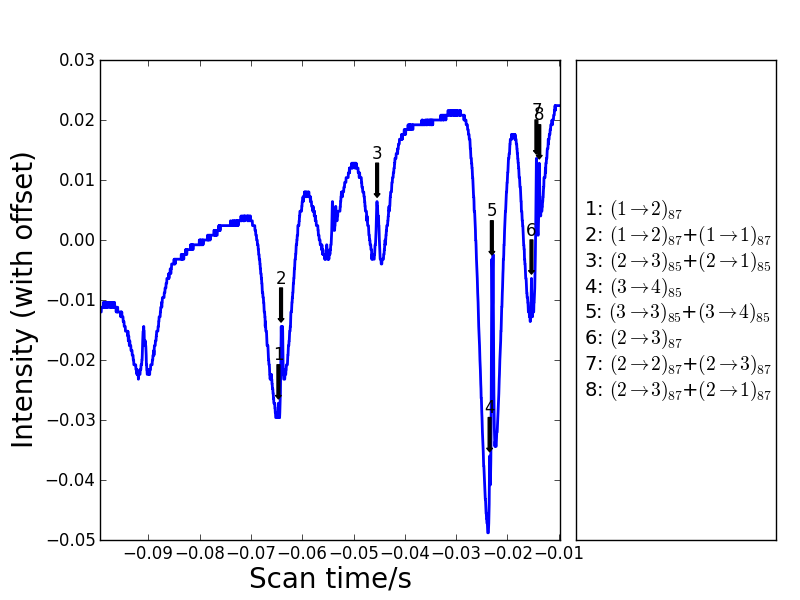
\includegraphics[width=6.2cm]{../all_data/4-18/20130418-14_12_48_probe.png}\\
    Probe beam intensity of the whole scan.
    \column{6cm}
    \visible<2>{
      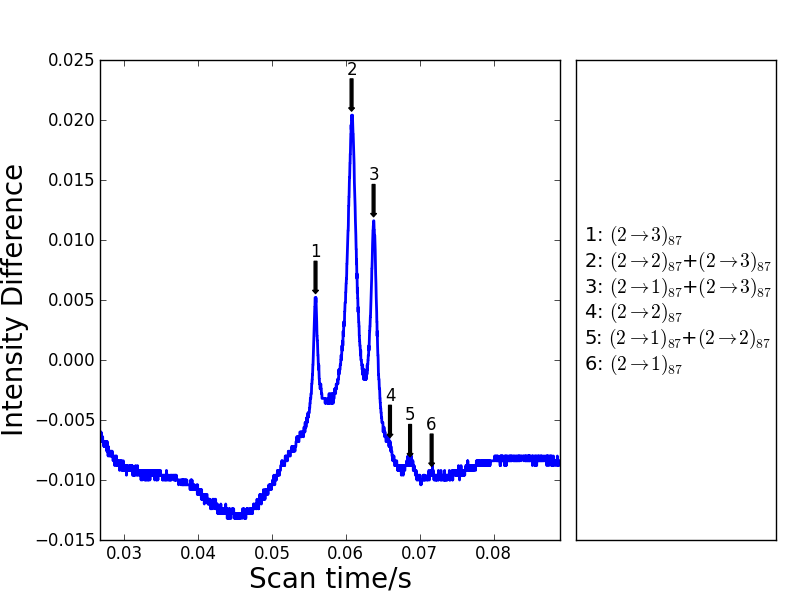
\includegraphics[width=6.2cm]{../all_data/4-18/20130418-12_52_13_balance.png}\\
      Difference between probe and reference beam intensity of the ${}^{87}Rb$ $F=2$ lines.
    }
  \end{columns}
\end{frame}

\begin{frame}{Hyperfine Structure Constants.}
  \begin{block}{Hyperfine Structure Constants.}
    \begin{center}
      \begin{tabular}{|c|c|c|c|c|}
        \hline
        Isotrope&Constant&Measured&Expected&Deviation\\\hline
        &$A_{5^2S_{1/2}}$&$0.986(40)GHz$&$1.0119GHz$&$0.6\sigma$\\\cline{2-5}
        ${}^{85}Rb$&$A_{5^2P_{3/2}}$&$24.44(81)MHz$&$25.0020(99)MHz$&$0.7\sigma$\\\cline{2-5}
        &$B_{5^2P_{3/2}}$&$32.2(4.8)MHz$&$25.790(93)MHz$&$1.3\sigma$\\\hline
        &$A_{5^2S_{1/2}}$&$3.285(65)GHz$&$3.4173GHz$&$2\sigma$\\\cline{2-5}
        ${}^{87}Rb$&$A_{5^2P_{3/2}}$&$84.58(52)MHz$&$84.7185(20)MHz$&$0.2\sigma$\\\cline{2-5}
        &$B_{5^2P_{3/2}}$&$16.03(80)MHz$&$12.4965(37)MHz$&$4\sigma$\\\hline
      \end{tabular}
    \end{center}
  \end{block}
\end{frame}

\def\timeleft{0:30->0:00}
\section{Conclusion.}
\begin{frame}{Conclusion.}
  \begin{block}{}
    \begin{itemize}[<+->]
    \item
      Observed Lamb dip.
    \item
      Measured hyperfine splitting and the hyperfine structure constants.
    \end{itemize}
  \end{block}
\end{frame}

\begin{frame}{}
\end{frame}

\begin{frame}{}
\end{frame}

\end{document}
